%% main.tex
%% Copyright 2022 skyleaworlder
%
% This work may be distributed and/or modified under the
% conditions of the LaTeX Project Public License, either version 1.3
% of this license or (at your option) any later version.
% The latest version of this license is in
%   http://www.latex-project.org/lppl.txt
% and version 1.3 or later is part of all distributions of LaTeX
% version 2003/12/01 or later.
%
% This work has the LPPL maintenance status "maintained".
%
% This Current Maintainer of this work is skyleaworlder.
%
% This work consists of all the *.tex and *.sty files in
%   https://github.com/TJ-CSCCG/Tongji-Beamer
\documentclass[aspectratio=169]{ctexbeamer}

\usepackage{amsthm}
\usepackage[style=gb7714-2015,backend=biber]{biblatex}
\addbibresource{reference.bib}
\setbeamertemplate{bibliography item}[text]

\usetheme{tongji}

% Customizations for URL and DOI fonts
\def\UrlFont{\ttfamily}
\DeclareFieldFormat{doi}{%
  \sffamily{DOI}\addcolon\space
  \ifhyperref
    {\href{https://doi.org/#1}{\nolinkurl{#1}}}
    {\nolinkurl{#1}}}


%Information to be included in the title page:
\title[Eternal-Night-Star-Bow]{Eternal-Night-Star-Bow: An Involution Detect System Implementation}
\subtitle{永夜星弓:内卷程度检测系统的一种实现}
\author[skyleaworlder, Cathy Mole]{
    1859527 skyleaworlder (Markdown Engineer), \\
    1852333 Cathy Mole (Eternal Night Archer)
}
\institute[IS, CS Dept., CEIE, Tongji Univ.]{
    Information Security, Computer Science and Technology Department, \\
    College of Electronic and Information Engineering (CEIE), \\
    Tongji University. \\
    同济大学\ 电子与信息工程学院\ 计算机科学与技术系\ 信息安全
}
\date{\today}

\begin{document}

\begin{frame}
    \titlepage
\end{frame}

%% introductioin.tex
%% Copyright 2022 skyleaworlder
%
% This work may be distributed and/or modified under the
% conditions of the LaTeX Project Public License, either version 1.3
% of this license or (at your option) any later version.
% The latest version of this license is in
%   http://www.latex-project.org/lppl.txt
% and version 1.3 or later is part of all distributions of LaTeX
% version 2003/12/01 or later.
%
% This work has the LPPL maintenance status "maintained".
% 
% This Current Maintainer of this work is skyleaworlder.
%
% This work consists of all the *.tex and *.sty files in
%   https://github.com/TJ-CSCCG/Tongji-Beamer
\section{引言}
    \begin{frame}
    % “无序列表” 与 “有序列表” 使用
    \frametitle{引言}
        \footnotesize
        \begin{block}{项目背景}
            \begin{itemize}
                \item 二十一世纪二十年代初,各大高校学生被卷入到一场声势浩大、旷日持久的内卷运动中。后世称之为 “永夜行动”,参加该类活动的学生被称为 “永夜村民”。
                \item 济勤学堂作为我校八大学堂之一,聚集了人工智能、大数据、计科、软工、信安、自动化等新工科专业,吸引了大批永夜村民。
                \item 当今时代不再内卷。但内卷仍是人们心中永远的痛。防范 “永夜村势力” 抬头,是当代每个优秀新青年的重要责任。
            \end{itemize}
        \end{block}
        
        \begin{block}{项目要素}
            \begin{enumerate}
                \item 开发内卷行为归因系统,通过历史数据分析得出二十年代初永夜行动的直接与间接原因。
                \item 开发内卷识别器,并在全校范围内构建内卷识别天网。
                \item 开发内卷信息收集与行为防范系统,避免永夜行动的重演。
            \end{enumerate}
        \end{block}
    \end{frame}


%% body.tex
%% Copyright 2022 skyleaworlder
%
% This work may be distributed and/or modified under the
% conditions of the LaTeX Project Public License, either version 1.3
% of this license or (at your option) any later version.
% The latest version of this license is in
%   http://www.latex-project.org/lppl.txt
% and version 1.3 or later is part of all distributions of LaTeX
% version 2003/12/01 or later.
%
% This work has the LPPL maintenance status "maintained".
%
% This Current Maintainer of this work is skyleaworlder.
%
% This work consists of all the *.tex and *.sty files in
%   https://github.com/TJ-CSCCG/Tongji-Beamer
\section{系统分析}
    % “图片文字并排” 示例
    \begin{frame}{内卷行为归因系统}
        \begin{columns}
            \column{.3\textwidth}
            \begin{figure}
                \centering 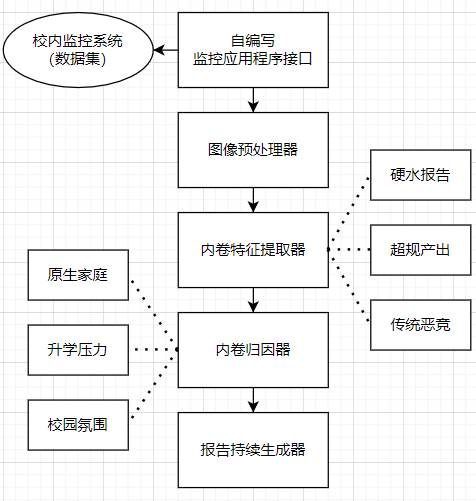
\includegraphics[width=.95\textwidth]{contents/figure/factor-analyzer.png}
                \caption{归因系统架构}
                \label{fig:factor-analyzer}
            \end{figure}

            \column{.6\textwidth}
            \begin{itemize}
                \item 校内监控系统:接入校内系统,使用过往录像作为归因系统模型训练数据集。
                \item 特征提取器:项目提出了数十种内卷特征类型。提取器要求人工为部分数据集标记标签。
                \item 内卷归因器:阅读历史文献,得出数十种内卷成因,构建内卷特征到成因的映射函数。
                \item 报告持续生成器:开发该系统的报告生成器,提升用户体验。
            \end{itemize}
        \end{columns}
    \end{frame}

    % “图片文字垂直” 示例
    \begin{frame}{内卷识别器}
        \begin{figure}
            \centering
            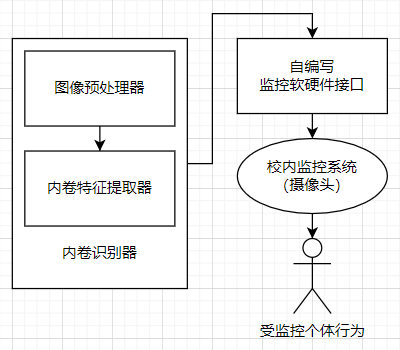
\includegraphics[width=.25\textwidth]{contents/figure/data-detector.png}
            \caption{识别器架构}
            \label{fig:data-detector}
        \end{figure}

        \begin{itemize}
            \item \small 复用归因系统中图像处理的特定阶段,编写软硬件接口,对接校内监控系统终端。
            \item \small 识别器特征提取结果将上传至我校私有云上,方便监管与处理。
        \end{itemize}
    \end{frame}

    % “多图片文字混合” 示例
    \begin{frame}{内卷信息收集与行为防范系统}
        \begin{columns}
            \column{.3\textwidth}
            \begin{figure}
                \centering
                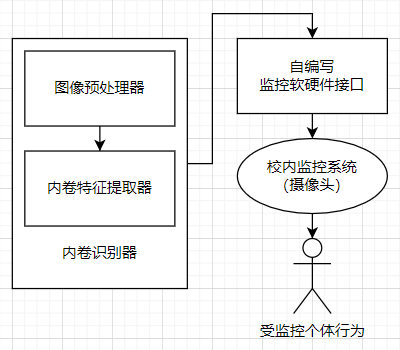
\includegraphics[width=\textwidth]{contents/figure/data-detector.png}
                \caption{识别器架构}
                \label{fig:data-detector-2}
            \end{figure}

            \column{.2\textwidth}
            \begin{figure}
                \centering
                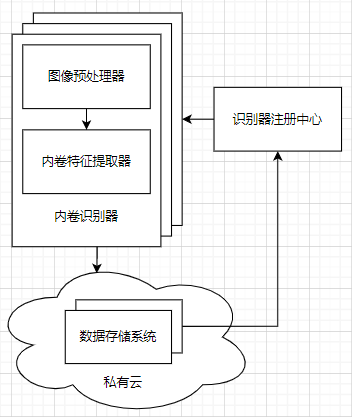
\includegraphics[width=\textwidth]{contents/figure/collector-part-1.png}
                \caption{信息收集系统}
                \label{fig:collector-part-1}
            \end{figure}

            \column{.25\textwidth}
            \begin{figure}
                \centering
                 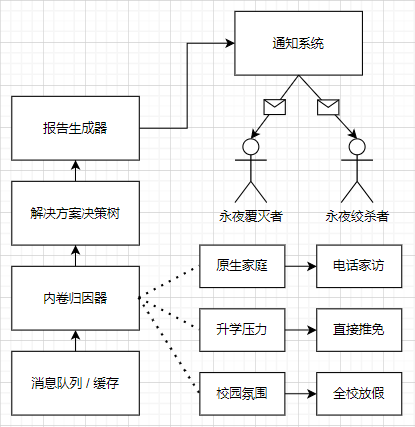
\includegraphics[width=\textwidth]{contents/figure/collector-part-2.png}
                \caption{行为防范系统}
                \label{fig:collector-part-2}
            \end{figure}
        \end{columns}

        \small 信息收集系统使用一个服务作为所有监控终端设备的“注册中心”,提供鉴权、心跳检查等能力;行为规范系统复用了归因系统中的特定因素分析阶段,以此作为决策树的判断基础。
    \end{frame}


\section{合理性分析}
    % “数学” 与 “公式” 示例
    \begin{frame}{专有名词释义}
        \begin{definition}[永夜势力]
            考虑一所高校,其中永夜村民的数量除以学生总数的值。
        \end{definition}
        \begin{theorem}[永夜定理]
            考虑一所高校,在不存在干涉的情况下,永夜势力在小于 1 前,恒呈指数型增长。
        \end{theorem}
        \begin{theorem}[永夜方程]
            考虑一所高校,人为干涉无效的概率为$x$。$x$是方程~\ref{eqn:x}~的解,其中$n$为全校学生总数。
        \begin{equation}\label{eqn:x}
            \begin{vmatrix}
            \begin{bmatrix}
                    x & \Phi(\pi) \\
                    \sum_{i = 1}^n x_i & \exp(x_i)
            \end{bmatrix}
            \begin{bmatrix}
                    1 & \cdots & n \\
                    x\Phi(e) & \cdots & x\Phi^n(e^n)
            \end{bmatrix}
            \end{vmatrix} = \dfrac{\pi}{x}
        \end{equation}
        \end{theorem}
    \end{frame}

    % “简单公式” 示例
    \begin{frame}{负载分析}
        系统在设计时进行了计算下沉,分离图像处理的多个步骤,实现计算的高效性。

        假设 $id \in [1850001, 1859999]$,识别器与分析器共有 $m$ 个机器,第 $i$ 个机器负责 $[1850001 + i \times \frac{9999}{m}, 1859999 + (i + 1) \times \frac{9999}{100}]$ 个单位。

        识别层机器会发送分析层机器需要的特定记录到存储中。存储中每个节点大小为 16~KB,由于一条记录占据 400~B 的空间,有:

        $$
        Node = \dfrac{16 \times 1024\operatorname{B}}{400 \operatorname{B}} \approx 16
        $$

        假设 $t$ 为一次操作所花费的时间,设单表大小为 $M$。在不进行计算分离时,消耗的时间 $T = Mt$。但在分离过后,全过程时间为:

        $$
        T' = \dfrac{M}{m} + \dfrac{9999}{m} \cdot t < Mt, \quad \text{if } m > \dfrac{1}{t} + \dfrac{9999}{M}
        $$
    \end{frame}


\section{组件设计}
    % “表格” 示例
    \begin{frame}{决策系统设计}
        \begin{table}[]
            \centering
            \begin{tabular}{c|c|c}
            \textbf{运行时间} & \textbf{实验组} & \textbf{对照组(单位 1)} \\
            \hline
                设计模式使用 vs. 不使用 & 1.1 & 1 \\
                Julia vs. Python & 0.7 & 1 \\
                负载均衡集群 vs. 单机 & 0.5 & 1 \\
                集群分布式缓存 vs. 无缓存 & 0.8 & 1 \\
            \end{tabular}
            \caption{各技术对决策系统的影响}
            \label{tab:tech-strategy}
        \end{table}
        
        \vspace{-1em}  % use vspace and hspace to adjust space
        
        \begin{columns}
            \small
            \column{.5\textwidth}
            \begin{itemize}
                \item 使用 Strategy 设计模式。
                \item 使用 Julia 高效计算矩阵乘法。
                \item 对归因系统暴露幂等性 API,使用计算集群增强计算能力。
            \end{itemize}

            \column{.5\textwidth}
            \begin{itemize}
                \item 采用负载均衡,平衡集群中各处理机的负载。
                \item 采用分布式缓存技术,加快集群整体对高频特殊输入的反应。
            \end{itemize}
        \end{columns}
    \end{frame}

    % “引用” 示例
    \begin{frame}{通知系统设计}
        著名哲人 skyleaworlder 有言:“内卷是可以被扼杀在摇篮中的。"\cite{involution} 只要在检测到疑似内卷行为后做到及时响应,由专业技术人员发起干涉,就有很相当概率阻止永夜势力的扩张。

        通知系统需要具备以下几个方面特性:
        \begin{enumerate}
            \item 即时性。内卷极易滋生壮大,通知专业技术人员的时间应该尽可能短。
            \item 高可用性。内卷行为来势汹汹,需要保证通知系统推送功能在高并发环境下的高可用性。
        \end{enumerate}

        自然卷说过:“内卷是凡人在挣扎中写下的血与泪的史诗。"\cite{undergrads_inv} 这份 “扭曲的美” 不应存于世间。
    \end{frame}

%% summary.tex
%% Copyright 2022 skyleaworlder
%
% This work may be distributed and/or modified under the
% conditions of the LaTeX Project Public License, either version 1.3
% of this license or (at your option) any later version.
% The latest version of this license is in
%   http://www.latex-project.org/lppl.txt
% and version 1.3 or later is part of all distributions of LaTeX
% version 2003/12/01 or later.
%
% This work has the LPPL maintenance status "maintained".
%
% This Current Maintainer of this work is skyleaworlder.
%
% This work consists of all the *.tex and *.sty files in
%   https://github.com/TJ-CSCCG/Tongji-Beamer
\section{总结}
    \begin{frame}{总结}
        “永夜星弓” 系统已在我校试运行 2 个月。试运行期间,上报内卷行为 300'000 起,成功制止 280'000 次轻微内卷行为、10'000 次中等内卷行为以及 10'000 次重度内卷行为。

        \begin{center}
            感谢在毕业设计实现过程中提供指导的老师们!

            感谢在这百余天中一直陪伴我的家人和同学们!

            感谢这个美丽的世界给了我从大学毕业的机会!
        \end{center}

        \begin{center}
            谢谢各位!请多多指教!
        \end{center}
    \end{frame}

\begin{frame}{参考文献}
    \printbibliography
\end{frame}

\end{document}
